\subsection{Distributional agreement and backbone sensitivity}\label{sec:distance}

The secondary distributional endpoint gives a more consistent result than selective category disagreement. Soft has lower squared distance than both controls in every tested seed, backbone and checkpoint state (Table~\ref{tab:distance}). For validation-selected Swin-T, mean distance is 0.09783 for Soft and 0.11571 for Uniform. This endpoint evaluates the complete probability vector on all 3,275 primary-test images, without confidence rejection. Supplementary Sect.~S2 provides the per-seed values for all five Swin-T and three ResNet-18 targets.

\begin{table}[t]\caption{Agreement with the complete crowd-vote distribution. Ten-category squared distances are averaged across three separate seeds on the same 3,275 test images. Lower is better; values are unscaled distance units, not percentages}\label{tab:distance}

\centering\small\begin{tabular}{llrrrrr}\toprule

Backbone & State & Soft & Uniform & Tie-Uniform & $\Delta_U$ & $\Delta_{TU}$\\\midrule

Swin-T & Selected & 0.09783 & 0.11571 & 0.11373 & -0.01787 & -0.01589\\

Swin-T & Epoch 12 & 0.09779 & 0.11699 & 0.11280 & -0.01920 & -0.01501\\

ResNet-18 & Selected & 0.11059 & 0.12303 & 0.11805 & -0.01244 & -0.00746\\

ResNet-18 & Epoch 12 & 0.11089 & 0.12259 & 0.11665 & -0.01170 & -0.00576\\

\bottomrule\end{tabular}\par\smallskip

$\Delta_U$ and $\Delta_{TU}$ are Soft minus Uniform and Soft minus Tie-Uniform. For each image, the score sums ten squared probability differences after adding three zero entries to the seven model outputs. It then averages across images. Vote distributions are not renormalized to the supported categories. Model probabilities are not combined across seeds.\par\end{table}

The adaptive ResNet-18 checks distinguish this distributional advantage from the selective result. For validation-selected ResNet-18, Soft-minus-Uniform disagreement is +0.173 pp, compared with -0.378 pp for Swin-T. All four ResNet-18 conditional intervals cross zero (Table~\ref{tab:backbones}), so these checks do not confirm Swin-T's selective advantage. Supplementary Sect.~S2 reports the per-seed contrasts and accompanying diagnostics. These are architecture-sensitivity checks using the same source images and adaptive study design, not independent-image confirmation.
\begin{table}[t]
\caption{Within-backbone Soft-minus-control disagreement at 80\% coverage (percentage points). Intervals condition on fitted models, three seeds, observed pixels and votes}\label{tab:backbones}
\centering\begin{tabular}{lllrr}\toprule
Backbone & State & Control & Difference & 95\% interval\\\midrule
Swin-T & selected & Uniform & -0.378 & [-0.644, -0.073]\\
Swin-T & selected & Tie-Uniform & -0.588 & [-0.830, -0.281]\\
Swin-T & epoch12 & Uniform & -0.317 & [-0.626, -0.050]\\
Swin-T & epoch12 & Tie-Uniform & -0.307 & [-0.585, -0.024]\\
ResNet-18 & selected & Uniform & +0.173 & [-0.167, +0.455]\\
ResNet-18 & selected & Tie-Uniform & +0.042 & [-0.258, +0.343]\\
ResNet-18 & epoch12 & Uniform & +0.170 & [-0.157, +0.467]\\
ResNet-18 & epoch12 & Tie-Uniform & +0.190 & [-0.126, +0.515]\\
\bottomrule\end{tabular}\par
\smallskip
ResNet comparisons are adaptive secondary robustness checks, not independent-image confirmation or architecture comparisons.\par
\end{table}


Figure~\ref{fig:backbones} brings the two endpoints together. Squared distance measures agreement across the complete annotation distribution, whereas category disagreement depends on the predicted category and, under confidence selection, the accepted-image set. Better distributional agreement can therefore coexist with little or no selective category advantage. The result concerns the tested source-dataset configurations; it does not establish deployment calibration or better external transfer.
\begin{figure}[tp]\centering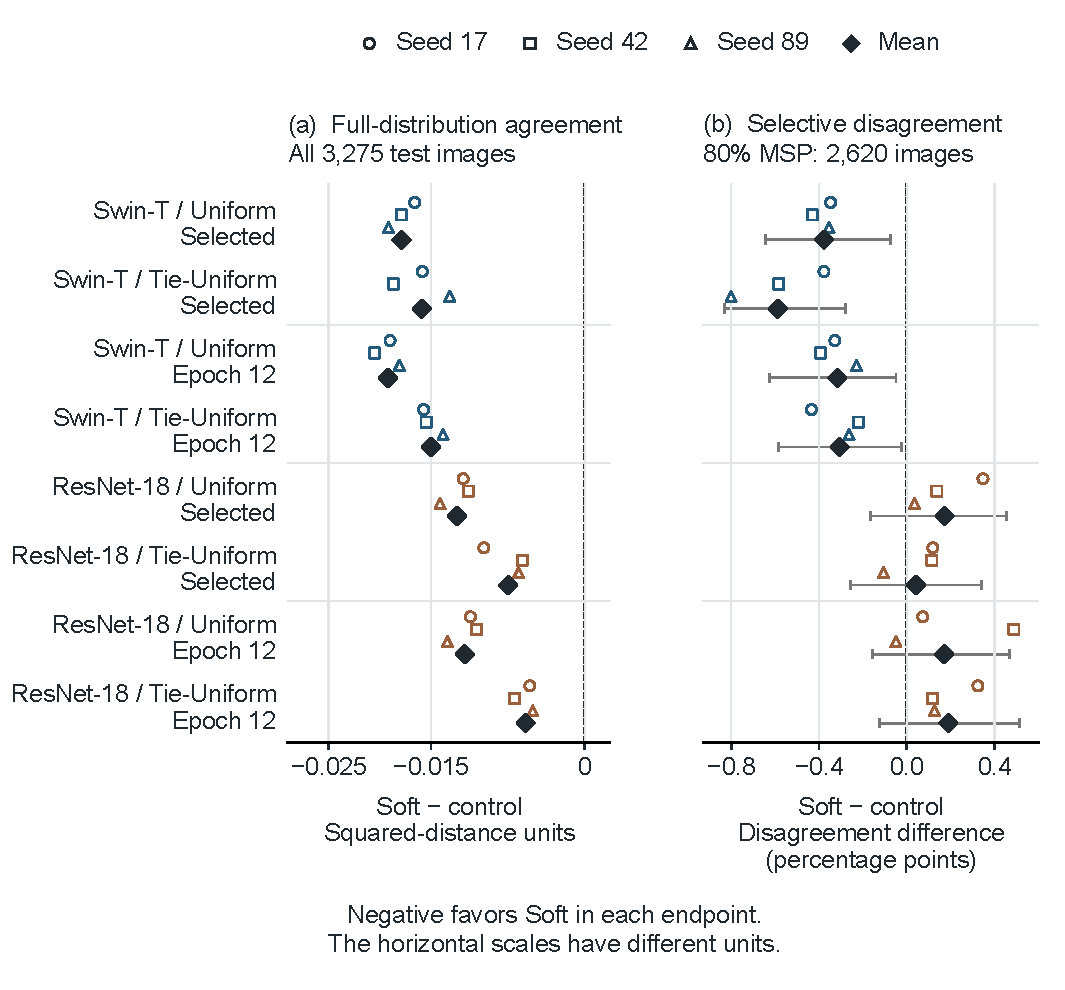
\includegraphics[width=\linewidth]{submission_reader_2026_10_13/source/figures/Fig7.pdf}
\caption{Distributional agreement and selective disagreement for Soft relative to the matched controls. (a) Ten-category squared-distance differences on all 3,275 primary-test images, in unscaled distance units. (b) Complete-vote disagreement differences at 80\% coverage using each model's ranking, in percentage points. Symbols show the three paired-seed contrasts and their mean. Bars in (b) are 95\% pixel-cluster bootstrap intervals conditional on the fitted models and observed votes; no interval is shown in (a). Both backbones and validation-selected and epoch-12 checkpoints are included. Negative values favor Soft. The panels use different units and scales}\label{fig:backbones}\end{figure}
